\documentclass{bmvc2k}

%% Enter your paper number here for the review copy
% \bmvcreviewcopy{??}

\title{PythonRobotics: a Python code collection of robotics algorithms}

% Enter the paper's authors in order
% \addauthor{Name}{email/homepage}{INSTITUTION_CODE}
\addauthor{Atsushi Sakai}{https://atsushisakai.github.io/}{1}

% Enter the institutions
% \addinstitution{Name\\Address}
\addinstitution{
 University of California, Berkeley\\
 Berkeley, USA
}


\runninghead{arXiv}{Artificial Intelligence}

% Any macro definitions you would like to include
% These are not defined in the style file, because they don't begin
% with \bmva, so they might conflict with the user's own macros.
% The \bmvaOneDot macro adds a full stop unless there is one in the
% text already.
\def\eg{\emph{e.g}\bmvaOneDot}
\def\Eg{\emph{E.g}\bmvaOneDot}
\def\etal{\emph{et al}\bmvaOneDot}

%------------------------------------------------------------------------- 
% Document starts here
\begin{document}

\maketitle

\begin{abstract}
This document demonstrates the format requirements for papers submitted
to the British Machine Vision Conference.  The format is designed for
easy on-screen reading, and to print well at one or two pages per sheet.
Additional features include: pop-up annotations for
citations~\cite{Authors06,Mermin89}; a margin ruler for reviewing; and a
greatly simplified way of entering multiple authors and institutions.

{\bf All authors are encouraged to read this document}, even if you have
written many papers before.  As well as a description of the format, the
document contains many instructions relating to formatting problems and
errors that are common even in the work of authors who {\em have}
written many papers before.
\end{abstract}

%------------------------------------------------------------------------- 
\section{Introduction}
\label{sec:intro}
The proceedings of BMVC are published only in electronic form, but it is still assumed
that readers of the papers may wish to print the paper.   This document
illustrates the required paper format, which is designed to read well either printed
with two pages per sheet (``2-up''), or on screen.  Note that printing with one page 
per sheet will produce a ``large print'' version, which in many cases is not what is desired.
To approximate the old BMVC format, print at one page per sheet, but do not choose
the option to ``scale to fit paper''.

\LaTeX\ users should use this template in order to prepare their paper.
Users of other packages should emulate the style and layout of this
example.  Note that best results will be achieved using {\tt pdflatex},
which is available in most modern distributions.

\subsection{Paper length: nine pages plus bibliography}
Paper length should not exceed 9~pages, {\em not counting} the bibliography.  {\bf Papers which are
 overlength will not be reviewed}.  This includes papers where the
margins and formatting are deemed to have been significantly altered from
those laid down by this style guide.  The reason such papers will not be
reviewed is that there is no provision for supervised revisions of
manuscripts.  The reviewing process cannot determine the suitability of the
paper for presentation in nine pages if it is reviewed in twelve.

The bibliography should begin immediately after the paper text.  It may
be of any length, within reason.  It should {\em not} include
annotations, figures, or any other paraphernalia intended to subvert the
paper length requirement.

\begin{figure}
\begin{tabular}{ccc}
\bmvaHangBox{\fbox{\parbox{2.7cm}{~\\[2.8mm]
\rule{0pt}{1ex}\hspace{2.24mm}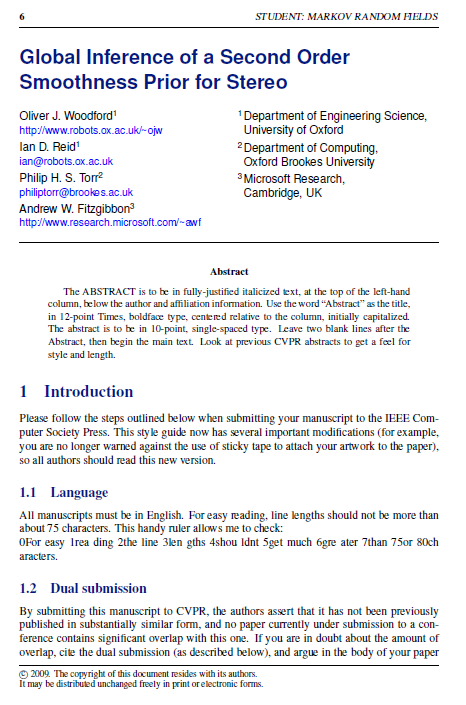
\includegraphics[width=2.33cm]{images/eg1_largeprint.png}\\[-0.1pt]}}}&
\bmvaHangBox{\fbox{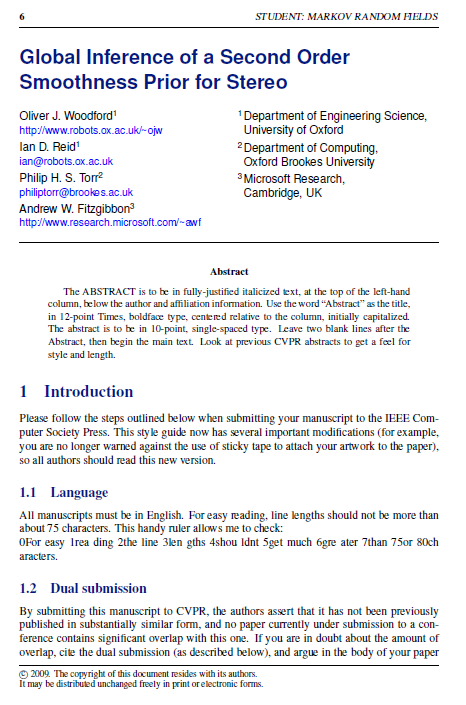
\includegraphics[width=2.8cm]{images/eg1_largeprint.png}}}&
\bmvaHangBox{\fbox{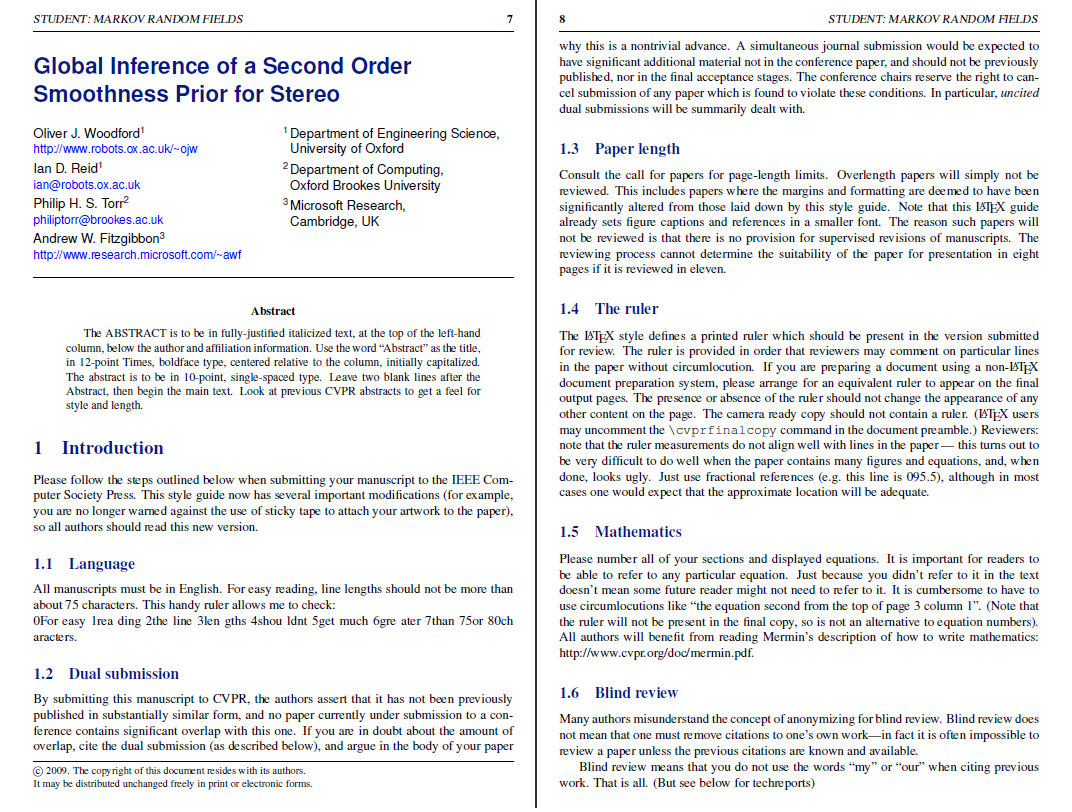
\includegraphics[width=5.6cm]{images/eg1_2up.png}}}\\
(a)&(b)&(c)
\end{tabular}
\caption{It is often a good idea for the first figure to attempt to
encapsulate the article, complementing the abstract.  This figure illustrates
the various print and on-screen layouts for which this paper format has
been optimized: (a) traditional BMVC print format; (b) on-screen
single-column format, or large-print paper; (c) full-screen two column, or
2-up printing. }
\label{fig:teaser}
\end{figure}

\subsection{Citations}
When citing a multi-author paper, you may save space by using ``{\em et
alia}'', shortened to ``\etal'' (not ``{\em et.\ al.}'' as ``{\em et}'' is
a complete word.)  The provided \verb'\etal' macro is a useful {\em aide
memoire} in this regard.  However, use it only when there are three or more
authors.  Thus, the following is correct: `` Frobnication has been trendy
lately.  It was introduced by Alpher~\cite{Alpher02}, and subsequently
developed by Alpher and Fotheringham-Smythe~\cite{Alpher03}, and Alpher
\etal~\cite{Alpher04}.''

This is incorrect: ``... subsequently developed by Alpher \etal~\cite{Alpher03} ...''
because reference~\cite{Alpher03} has just two authors.  If you use the
\verb'\etal' macro, then you need not worry about double periods
when used at the end of a sentence as in Alpher \etal.

%For this citation style, keep multiple citations in numerical (not
%chronological) order, so prefer
We use {\tt natbib}, so citations in random order are nicely sorted:
 \cite{Alpher03,Alpher02,Authors06b,Authors06}.  However, we don't use the
compress option, as we want each reference to have its own hyperlink and
popup window.

%------------------------------------------------------------------------- 
\subsection{Footnotes}

Please use footnotes\footnote {This is what a footnote looks like.  It
often distracts the reader from the main flow of the argument.} sparingly.
Indeed, try to avoid footnotes altogether and include necessary peripheral
observations in 
the text (within parentheses, if you prefer, as in this sentence).  If you
wish to use a footnote, place it at the bottom of the column on the page on
which it is referenced. Use Times 8-point type, single-spaced.


\begin{figure*}
\begin{center}
\fbox{\rule{0pt}{2in} \rule{.9\linewidth}{0pt}}
\end{center}
   \caption{Example of a short caption, which should be centered.}
\label{fig:short}
\end{figure*}

\begin{table}
\begin{center}
\begin{tabular}{|l|c|}
\hline
Method & Frobnability \\
\hline\hline
Theirs & Frumpy \\
Yours & Frobbly \\
Ours & Makes one's heart Frob\\
\hline
\end{tabular}
\end{center}
\caption{Results.   Ours is better.}
\end{table}

\subsection{Mathematics}

Please number all of your sections and displayed equations.  It is
important for readers to be able to refer to any particular equation.  Just
because you didn't refer to it in the text doesn't mean some future reader
might not need to refer to it.  It is cumbersome to have to use
circumlocutions like ``the equation second from the top of page 3 column
1''.  (Note that the ruler will not be present in the final copy, so is not
an alternative to equation numbers).  All authors will benefit from reading
Mermin's description~\cite{Mermin89} of how to write mathematics.


%------------------------------------------------------------------------- 
\subsection{References}

List and number all bibliographical references in 9-point Times,
single-spaced, at the end of your paper. When referenced in the text,
enclose the citation number in square brackets, for
example~\cite{Authors06}.  Where appropriate, include the name(s) of
editors of referenced books.


%------------------------------------------------------------------------
\subsection{Acknowledgments}

I appreciate contributors: Daniel Ingram, Joe Dinius, and Karan Chawla.

\bibliography{egbib}
\end{document}
